\chapter{Spatial Data}\label{ch:spatial-data}
Spatial Data is an important concept in this project. It is used throughout the whole project and in this chapter the most
important terms \& notations will be introduced and explained thoroughly so that the users understand what spatial data is,
its usage and the way it is represented by standardized formats.\\
\newline
Geospatial data is information that describes objects, events or other features with a location on
or near the surface of the earth.
Geospatial data typically combines location information (usually coordinates on the earth) and attribute information
(the characteristics of the object, event or phenomena concerned) with temporal information
(the time or life span at which the location and attributes exist).
The location provided may be static in the short term (for example, the location of a piece of equipment,
an earthquake event, children living in poverty) or dynamic
(for example, a moving vehicle or pedestrian, the spread of an infectious disease). \cite{IBMGeoSpatialData}\\
\newline
A lot of organizations have contributed to standardizing the way of representing geospatial data and ways of
exchanging such data between two parties. In this project, you will encounter a lot of notations such as:
\begin{itemize}
    \item Simple Features (or Simple Feature Access)
    \item Latitude/Longitude
    \item Well-Known Text (or WKT)
    \item GeoJSON
\end{itemize}

\begin{figure}[H]
    \centering
    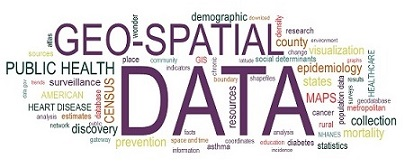
\includegraphics[width=10cm]{./Figures/Spatial_Data/geospatial_data.jpg}
    \caption{Geospatial data, adopted from \href{https://www.cdc.gov/dhdsp/maps/gisx/resources/geo-spatial-data.html}{\textit{Centers for Disease Control and Prevention}} \cite{CDC}}
\end{figure}
\section{Simple Features}
Simple Features (officially Simple Feature Access) is a set of standards that specify
a common storage and access model of geographic feature made of mostly
two-dimensional geometries (point, line, polygon, multi-point, multi-line, etc.)
used by geographic information systems.
It is formalized by both the \href{https://www.ogc.org/}{Open Geospatial Consortium (OGC)} and the
\href{https://www.iso.org/home.html}{International Organization for Standardization (ISO)}. \cite{SimpleFeaturesWiki}\\
\newline
This set of standards on how to represent real world objects is important in this project because it is used throughout
both of the extensions as means of representing geometry objects and then smoothing the process of working with such objects.
Some of the Java libraries used in this project also use such standards to represent geometry objects.
\begin{figure}[H]
    \centering
    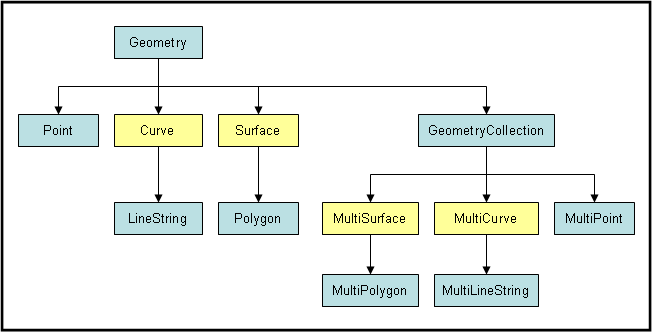
\includegraphics[width=\linewidth]{./Figures/Spatial_Data/simple_features.png}
    \caption{OGC Simple Features, the geometry classes usually used are shown in the blue, adopted from \href{http://gsp.humboldt.edu/Websites/BlueSpray/STUsersGuide/Scripting/Script_SimpleFeatures.html}{\textit{SchoonerTurtles Inc.}} \cite{SchoonerTurtles}}
\end{figure}
\section{Encoding Points}
The \textbf{Latitude} and \textbf{Longitude} is a widely popular concept in geospatial data, maybe because it is easier
to be comprehended and used by the users. A latitude and longitude combination of values is able to represent any exact location on the map
of the Earth\'s surface.\\
\newline
Here\'s an example of a latitude and longitude combination that represent the exact location of one of the OST Rapperswil
Mensas location: \mintinline{bash}{47.2231300, 8.8162990} as taken from the following
\href{http://overpass-turbo.osm.ch/?Q=area%0A%20%20%5B%22name%22%3D%22Rapperswil-Jona%22%5D-%3E.a%3B%0A(%0A%09nwr%0A%20%20%20%20(area.a)%0A%20%20%20%20%5B%22name%22%3D%22Mensa%20OST%20Campus%20Rapperswil%20Jona%22%5D%3B%0A)%3B%0Aout%20center%3B&C=47.22281;8.81693;19}{query} in
\href{http://overpass-turbo.osm.ch/}{Overpass Turbo CH}.
\subsection{Latitude}
Horizontal mapping lines on Earth are lines of latitude.
They are known as "parallels" of latitude, because they run parallel to the equator.
One simple way to visualize this might be to think about having imaginary horizontal "hula hoops" around the earth,
with the biggest hoop around the equator, and then progressively smaller ones stacked above and
below it to reach the North and South Poles. \cite{JourneyNorthLatitudeLongitude}
\subsection{Longitude}
Longitude lines are a numerical way to show/measure how far a location is east or west of a universal vertical line called the
Prime Meridian.
This Prime Meridian line runs vertically, north and south, right over the British Royal Observatory in
Greenwich England, from the North Pole to the South Pole.
As the vertical starting point for longitude, the Prime Meridian is numbered 0 degrees longitude. \cite{JourneyNorthLatitudeLongitude}
\section{Spatial Objects as Well-Known Text (WKT)}
Geospatial objects can be represented using the mark-up language called \href{https://www.ogc.org/standards/wkt-crs}{Well-Known Text (WKT)}.
They are not case-sensitive and are used to represent geometry objects such as: Points, LineStrings, Polygons, MultiPoints etc.\\
\newline
The formats were originally defined by the Open Geospatial Consortium (OGC) and described in their Simple Feature Access.
In this project, WKT strings are widely used and processed to e.g. represent OSM objects (converted to Simple Features) as strings and also for exporting
WKT strings to valid GeoJSON. \cite{OGCWKT}\\
\newline
Here's some examples of WKT strings, adopted from \href{https://www.vertica.com/docs/9.3.x/HTML/Content/Authoring/AnalyzingData/Geospatial/Spatial_Definitions/WellknownTextWKT.htm}{Vertica\'s Well-Known Text (WKT) documentation}: \cite{VerticaWKT}
\begin{itemize}
    \item \mintinline{bash}{POINT(1 2)} - Represents the point (1,2)
    \item \mintinline{bash}{MULTIPOINT(0 0,1 1)} - Represents a set made up of points (0,0) and (1,1)
    \item \mintinline{bash}{LINESTRING(1.5 2.45,3.21 4)} - Represents the line from the point (1.5,2.45) to the point (3.21,4)
    \item \mintinline{bash}{POLYGON((1 2,1 4,3 4,3 2,1 2))} - Represents a polygon (0.5 0.5,5 0,5 5,0 5,0.5 0.5) with a hole in it (1.5 1,4 3,4 1,1.5 1).
\end{itemize}
\section{Geospatial Data in GeoJSON}
Another format of representing Geospatial Data using the famous JSON format is the \href{https://datatracker.ietf.org/doc/html/rfc7946}{GeoJSON format}.
It is designed to represent simple geographical features, along with their non-spatial attributes.\\
\newline
GeoJSON is a geospatial data interchange format based on JavaScript
Object Notation (JSON).  It defines several types of JSON objects and
the manner in which they are combined to represent data about
geographic features, their properties, and their spatial extents.
GeoJSON uses a geographic coordinate reference system, World Geodetic
System 1984, and units of decimal degrees. \cite{WhatIsGeoJSON}\\
\newline
In this project, GeoJSON is used in the \textbf{GeoJSON Export} extension in order to export OpenRefine data to the
GeoJSON format. More information on the export process and details is described in the \hyperref[ch:the-geojson-export-extension]{GeoJSON Export Extension} chapter.